\begin{figure}
\centering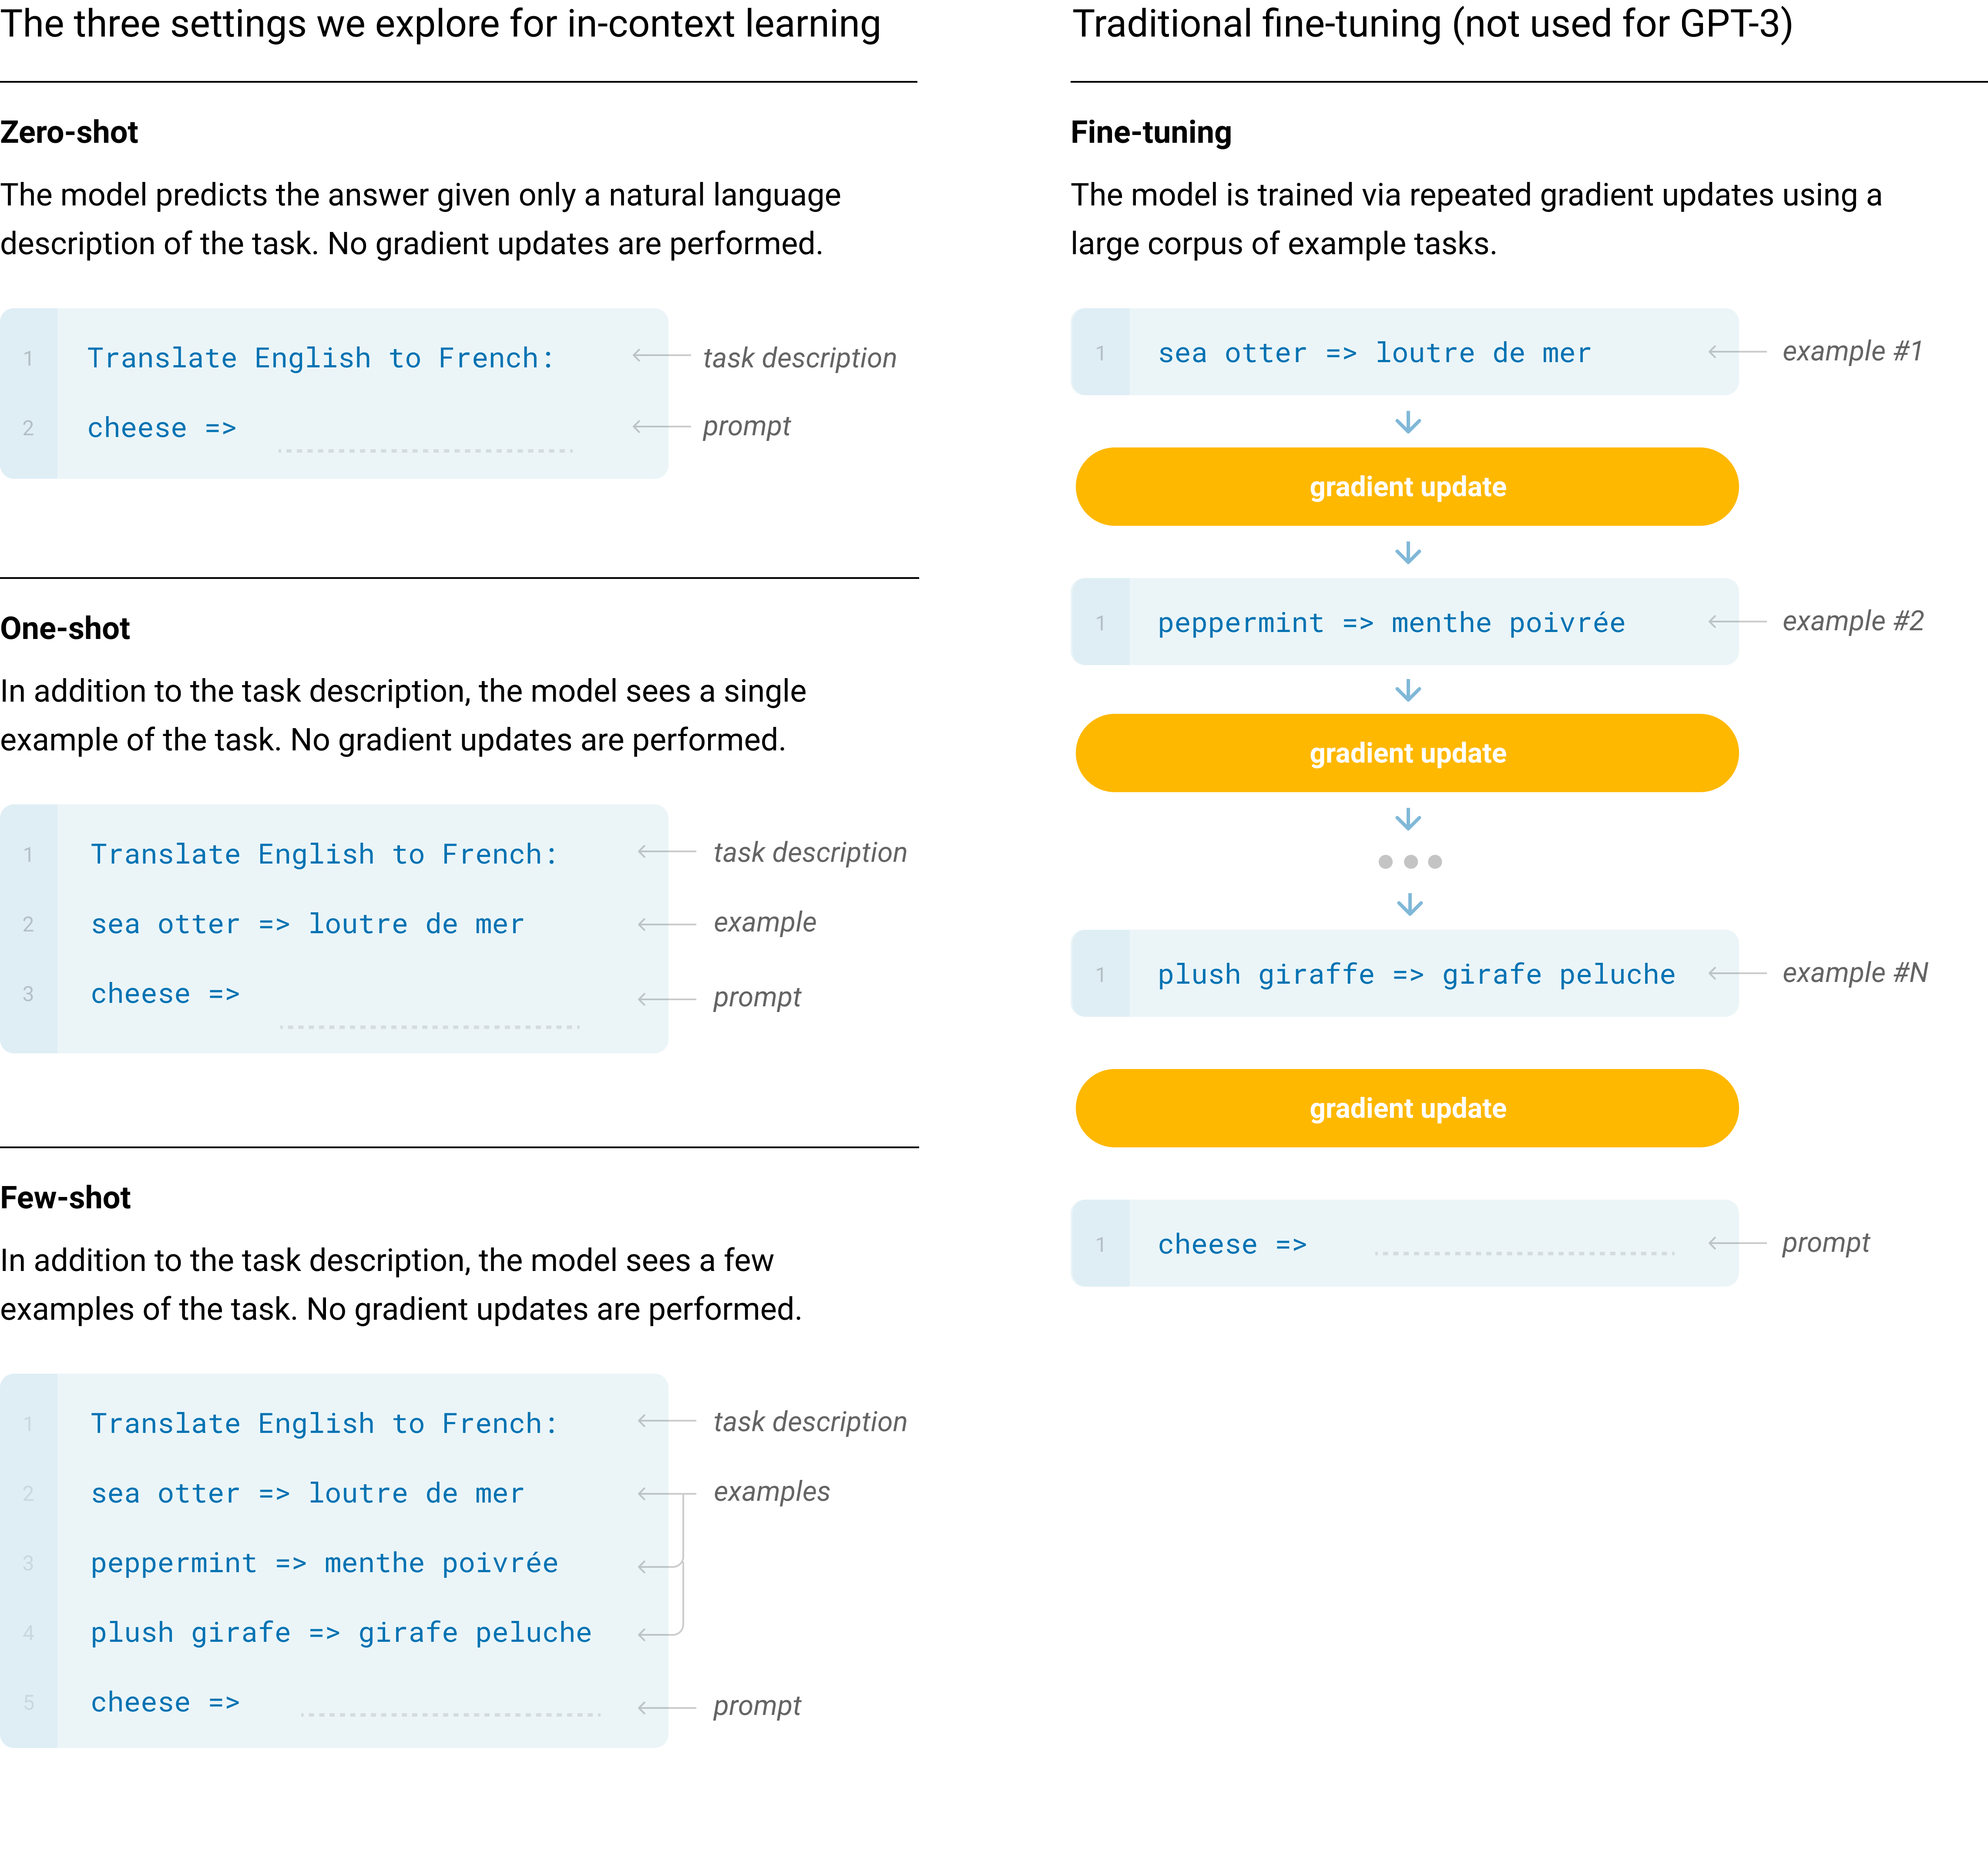
\includegraphics[width=0.8\linewidth]{figures/eval_strategies.png}
\caption{\textbf{Zero-shot, one-shot and few-shot, contrasted with traditional fine-tuning}. The panels above show four methods for performing a task with a language model -- fine-tuning is the traditional method, whereas zero-, one-, and few-shot, which we study in this work, require the model to perform the task with only forward passes at test time. We typically present the model with a few dozen examples in the few shot setting. Exact phrasings for all task descriptions, examples and prompts can be found in Appendix \ref{appendix:task_phrasing}.
}
\label{figure:eval strategies}
\end{figure}